\documentclass[tikz]{standalone}

\begin{document}

\tikzset{every picture/.style={line width=0.75pt}} %set default line width to 0.75pt        

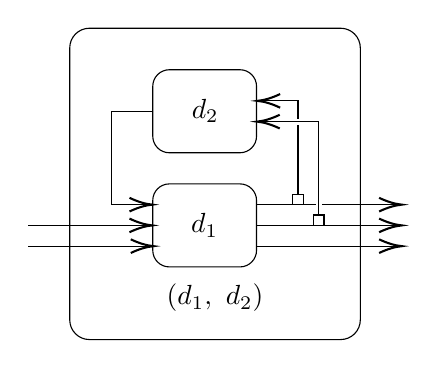
\begin{tikzpicture}[x=0.75pt,y=0.75pt,yscale=-1,xscale=1]
  %uncomment if require: \path (0,193); %set diagram left start at 0, and has height of 193

  %Shape: Boxed Line [id:dp7368791975286189] 
  \draw	 (140,90) -- (140,45) -- (122.44,45) ;
  \draw [shift={(120.44,45)}, rotate = 360] [color={rgb, 255:red, 0; green, 0; blue, 0 }	][line width=0.75]
  (10.93,-3.29) .. controls (6.95,-1.4) and (3.31,-0.3) .. (0,0) .. controls (3.31,0.3) and (6.95,1.4)
  .. (10.93,3.29)
  ;
  %Straight Lines [id:da16664242951426234] 
  \draw [color={rgb, 255:red, 255; green, 255; blue, 255 }	,draw opacity=1 ][line width=2.25]	(120,55) -- (148.67,55)
  ;
  %Straight Lines [id:da6703194392261191] 
  \draw	 (120,95) -- (188,95) ;
  \draw [shift={(190,95)}, rotate = 180] [color={rgb, 255:red, 0; green, 0; blue, 0 }	][line width=0.75]
  (10.93,-3.29) .. controls (6.95,-1.4) and (3.31,-0.3) .. (0,0) .. controls (3.31,0.3) and (6.95,1.4)
  .. (10.93,3.29)
  ;
  %Straight Lines [id:da4174191896870494] 
  \draw [color={rgb, 255:red, 255; green, 255; blue, 255 }	,draw opacity=1 ][line width=2.25]	(150,50) -- (150,100) ;
  %Rounded Rect [id:dp7550223310785882] 
  \draw	(70,38) .. controls (70,33.58) and (73.58,30) .. (78,30) -- (112,30) .. controls (116.42,30)
  and (120,33.58) ..
  (120,38) -- (120,62) .. controls (120,66.42) and (116.42,70) .. (112,70) -- (78,70) .. controls (73.58,70)
  and
  (70,66.42) .. (70,62) -- cycle ;
  %Straight Lines [id:da5327288968036628] 
  \draw	 (120,105) -- (188,105) ;
  \draw [shift={(190,105)}, rotate = 180] [color={rgb, 255:red, 0; green, 0; blue, 0 }	][line width=0.75]
  (10.93,-3.29) .. controls (6.95,-1.4) and (3.31,-0.3) .. (0,0) .. controls (3.31,0.3) and (6.95,1.4)
  .. (10.93,3.29)
  ;
  %Rounded Rect [id:dp6106553970186992] 
  \draw	(70,93) .. controls (70,88.58) and (73.58,85) .. (78,85) -- (112,85) .. controls (116.42,85)
  and (120,88.58) ..
  (120,93) -- (120,117) .. controls (120,121.42) and (116.42,125) .. (112,125) -- (78,125) .. controls
  (73.58,125) and
  (70,121.42) .. (70,117) -- cycle ;
  %Rounded Rect [id:dp9737700137701875] 
  \draw	(30,19.5) .. controls (30,14.25) and (34.25,10) .. (39.5,10) -- (160.5,10) .. controls
  (165.75,10) and
  (170,14.25) .. (170,19.5) -- (170,150.5) .. controls (170,155.75) and (165.75,160) .. (160.5,160) --
  (39.5,160) ..
  controls (34.25,160) and (30,155.75) .. (30,150.5) -- cycle ; %Straight Lines [id:da37580228093374113] 
  \draw	 (10,105) -- (67.71,105) ; \draw [shift={(69.71,105)}, rotate = 180] [color={rgb, 255:red, 0; green, 0; blue, 0 } ][line width=0.75]
  (10.93,-3.29) .. controls (6.95,-1.4) and (3.31,-0.3) .. (0,0) .. controls
  (3.31,0.3) and (6.95,1.4) .. (10.93,3.29) ;  \draw	 (10,115) -- (68.35,115) ;%Straight Lines [id:da08332712024418076] 
  \draw [shift={(70.35,115)}, rotate = 180] [color={rgb, 255:red, 0; green, 0; blue, 0 } ][line width=0.75]
  (10.93,-3.29) .. controls (6.95,-1.4) and (3.31,-0.3) .. (0,0) .. controls (3.31,0.3) and (6.95,1.4)
  .. (10.93,3.29) ;  \draw	 (70.22,50) -- (50,50) -- (50,95) -- (67.74,95) ; \draw [shift={(69.74,95)}, rotate = 180] [color={rgb, 255:red, 0; green, 0; blue, 0 }  ][line width=0.75]%Shape: Boxed Line [id:dp0022463151100715617] 
  (10.93,-3.29) ..
  controls (6.95,-1.4) and (3.31,-0.3) .. (0,0) .. controls (3.31,0.3) and (6.95,1.4) .. (10.93,3.29) ;
   \draw	 (150,100) -- (150,55) -- (122.22,55) ; \draw [shift={(120.22,55)}, rotate = 360] [color={rgb, 255:red, 0; green, 0; blue, 0 } ][line width=0.75]%Shape: Boxed Line [id:dp712757888130485] 
  (10.93,-3.29) .. controls (6.95,-1.4) and
  (3.31,-0.3) .. (0,0) .. controls (3.31,0.3) and (6.95,1.4) .. (10.93,3.29) ;
   \draw	(137.5,90) -- (142.5,90) -- (142.5,95) -- (137.5,95) -- cycle ; %Straight Lines [id:da043881539950311854] %Shape: Rectangle [id:dp41508981481880025] 
  \draw	 (120,115) -- (151.41,115) -- (188,115) ; \draw [shift={(190,115)}, rotate = 180] [color={rgb, 255:red, 0; green, 0; blue, 0 }  ][line width=0.75]
  (10.93,-3.29) .. controls (6.95,-1.4) and (3.31,-0.3) .. (0,0) .. controls
  (3.31,0.3) and (6.95,1.4) .. (10.93,3.29) ;  \draw	(147.5,100) -- (152.5,100) -- (152.5,105) -- (147.5,105) -- cycle%Shape: Rectangle [id:dp4568859222640498] 
  ;

  % Text Node
  \draw (95.25,50) node	[align=left] {$\displaystyle d_{2}$};
  % Text Node
  \draw (95,105) node   [align=left] {$\displaystyle d_{1}$};
  % Text Node
  \draw (100,140) node   [align=left] {$\displaystyle \Recursive( d_{1} ,\ d_{2})$};

\end{tikzpicture}
\end{document}
